\documentclass[11pt]{article}

\usepackage[french]{babel}
\usepackage[utf8]{inputenc}
\usepackage[T1]{fontenc}
\usepackage{lmodern}
\usepackage{amsmath,amssymb}
\usepackage{graphicx}
\usepackage{tikz}
\usetikzlibrary{positioning,arrows.meta,calc,shadows,shapes.geometric,fit}
\usepackage{booktabs}
\usepackage[margin=2.5cm]{geometry}
\usepackage{hyperref}
\usepackage{float}
\usepackage{caption}
\usepackage{xcolor}
\usepackage{listings}
\usepackage{cite}
\usepackage{placeins}
\usepackage{array}
\usepackage{longtable}

\graphicspath{{figures/}}
\linespread{1.08}
\sloppy
\hypersetup{
  colorlinks=true,
  linkcolor=black,
  citecolor=black,
  urlcolor=blue
}

\newcommand{\github}{\url{https://github.com/JudicaelMAKWIZA/imprecise-movie-fuzzy-recommender}}

\lstset{
  basicstyle=\ttfamily\small,
  columns=fullflexible,
  frame=single,
  breaklines=true,
  showstringspaces=false
}

\begin{document}

\thispagestyle{empty}
\begin{center}
  {\bfseries\small REPUBLIQUE DEMOCRATIQUE DU CONGO} \\[2pt]
  {\bfseries\small UNIVERSITE DE KINSHASA} \\[6pt]
  
\includegraphics[width=0.14\textwidth]{images.png} \\[6pt]
  {\small FACULTE DES SCIENCES ET TECHNOLOGIES \\ Mention Mathematiques, Statistique et Informatique} \\[2pt]
  {\small B.P. 190 KINSHASA XI} \\[6pt]
  {\small Master 2} \\[6pt]
  {\bfseries\large LOGIQUE FLOUE EN INTELLIGENCE ARTIFICIELLE} \\[12pt]
  {\Large\bfseries Systeme de Recommandation Flou base sur les Preferences Imprecises des Utilisateurs} \\[8pt]
  {\normalsize\itshape Application au catalogue MovieLens via une inference de Mamdani} \\[14pt]
  {\normalsize Sujet 12} \\[12pt]
  {\normalsize DUASENGE MAYANO Brummel} \\[10pt]
  {\normalsize Juin 2026}
\end{center}

\vspace{10pt}
\begin{abstract}
Ce rapport presente la conception, l'implementation et l'evaluation d'un systeme de recommandation de films fonde sur la logique floue. Le probleme traite est celui des preferences utilisateur imprecises, souvent exprimees sous forme linguistique ou intervalle plutot que par une note numerique unique. Le systeme propose combine un pre-filtrage par genre, une inference de Mamdani et une defuzzification par centroide afin de produire un score interpretable pour chaque film candidat. L'application est realisee sur le jeu de donnees MovieLens et exposee a travers une interface en ligne de commande et une interface graphique Tkinter.
\end{abstract}

\newpage
\tableofcontents
\newpage

\input{sections/01_introduction}
\section{Cadre theorique}

Cette section introduit les notions mobilisees dans le systeme developpe. Elle part de la definition d'un ensemble flou, puis montre comment les variables linguistiques et l'inference de Mamdani permettent de manipuler des preferences imprecises.

\subsection{Logique floue et ensembles flous}

Dans la theorie classique des ensembles, un element appartient ou n'appartient pas a un ensemble. La logique floue propose une generalisation : un ensemble flou $\tilde{A}$ defini sur un univers $X$ est caracterise par une fonction d'appartenance
\[
\mu_A : X \rightarrow [0,1],
\]
ou $\mu_A(x)$ mesure le degre auquel $x$ appartient a $\tilde{A}$ \cite{zadeh1965,klir1995}. Ainsi, une note moyenne de film peut appartenir partiellement au terme \emph{bonne} et partiellement au terme \emph{excellente}.

Deux formes simples sont utilisees dans ce projet. Une fonction triangulaire de parametres $(a,b,c)$ est donnee par :
\[
\mu(x)=
\begin{cases}
0, & x \leq a,\\
\frac{x-a}{b-a}, & a < x \leq b,\\
\frac{c-x}{c-b}, & b < x < c,\\
0, & x \geq c.
\end{cases}
\]
Une fonction trapezoidale de parametres $(a,b,c,d)$ est donnee par :
\[
\mu(x)=
\begin{cases}
0, & x \leq a,\\
\frac{x-a}{b-a}, & a < x \leq b,\\
1, & b < x \leq c,\\
\frac{d-x}{d-c}, & c < x < d,\\
0, & x \geq d.
\end{cases}
\]
Ces fonctions sont simples, mais suffisantes pour obtenir des zones de transition progressives entre termes voisins.

\subsection{Variables linguistiques}

Une variable linguistique associe un univers numerique a un ensemble de termes interpretables \cite{zadeh1975}. Par exemple, la variable \texttt{genre\_preference} est definie sur $[0,1]$ avec les termes \emph{faible}, \emph{moyenne} et \emph{forte}. La granularite choisie influence directement la lisibilite des regles : peu de termes rendent le systeme compact, tandis qu'un nombre plus eleve de termes permet une decision plus fine.

Dans ce travail, les variables linguistiques ne sont pas seulement descriptives. Elles sont les entrees et la sortie du moteur Mamdani : preference de genre, note moyenne, popularite et score de recommandation. Ce lien entre langage et calcul ouvre naturellement la voie a la representation des preferences imprecises.

\subsection{Preferences imprecises}

Une preference imprecise designe une information utilisateur dont la valeur exacte n'est pas connue ou n'est pas exprimee sous forme ponctuelle. Le systeme supporte trois modes. Le mode linguistique permet de saisir un terme comme \emph{forte}. Le mode intervalle permet de saisir une plage telle que $0.6..0.9$. Le mode crisp accepte une valeur numerique unique dans $[0,1]$ lorsque l'utilisateur veut etre precis.

Pour relier ces modes au calcul flou, le systeme utilise une projection vers des degres d'appartenance. Un terme linguistique est transforme en zone d'incertitude par un alpha-cut a 0.5 ; un intervalle est projete en prenant, pour chaque terme, le degre maximal atteint dans la plage. Cette strategie evite de reduire immediatement une expression vague a un seul nombre.

\subsection{Inference de Mamdani}

L'inference de Mamdani est un modele de raisonnement flou fonde sur des regles de la forme \emph{si... alors...} \cite{mamdani1975}. Dans ce projet, le processus suit quatre etapes : fuzzification des entrees, activation des regles, agregation des sorties et defuzzification.

Pour une regle comportant plusieurs antecedents, le degre d'activation est calcule par un operateur minimum. Les sorties activees sont ensuite agregees par maximum. Enfin, le score crisp est obtenu par la methode du centroide :
\[
z^*=\frac{\int z\cdot \mu(z)\,dz}{\int \mu(z)\,dz}.
\]
Ce choix conserve une interpretation graphique claire : le score final correspond au centre de gravite de la surface floue agregee.

\subsection{Systemes de recommandation et MovieLens}

MovieLens est un ensemble de donnees de reference pour l'etude des systemes de recommandation \cite{harper2015}. La version utilisee dans ce projet contient quatre fichiers principaux : \texttt{movies.csv}, \texttt{ratings.csv}, \texttt{tags.csv} et \texttt{links.csv}. Les films apportent les titres et genres, les notes permettent de calculer des moyennes et des popularites, les tags donnent des annotations libres, et les liens fournissent des identifiants externes.

Le projet exploite principalement les genres, les notes moyennes et le nombre de notes. Ces informations sont suffisantes pour construire une premiere version interpretable du systeme. La section suivante montre comment elles sont organisees dans une architecture logicielle modulaire.

\section{Architecture du systeme}

L'architecture du systeme separe clairement les responsabilites : chargement des donnees, calcul flou, recommandation, evaluation, visualisation et interfaces. Cette separation facilite les tests et rend le comportement du moteur plus reproductible.

\begin{figure}[H]
\centering
\resizebox{0.92\textwidth}{!}{%
\begin{tikzpicture}[
  >=Stealth,
  layer/.style={draw=black!60, rounded corners, thick, minimum width=4.0cm, minimum height=1.0cm, align=center, fill=blue!8, drop shadow},
  service/.style={draw=black!55, rounded corners, thick, minimum width=3.4cm, minimum height=0.85cm, align=center, fill=green!9},
  arr/.style={->, thick}
]
  \node[layer] (data) {data\_manager\\chargement et features};
  \node[layer, right=1.8cm of data] (fuzzy) {fuzzy\\variables, regles, inference};
  \node[layer, right=1.8cm of fuzzy] (rec) {recommender\\profil, scoring, Top-N};
  \node[service, below=1.2cm of fuzzy] (eval) {evaluation\\metriques};
  \node[service, below=1.2cm of data] (vis) {visualization\\courbes};
  \node[service, below=1.2cm of rec] (ui) {ui\\CLI et GUI};
  \draw[arr] (data) -- (fuzzy);
  \draw[arr] (fuzzy) -- (rec);
  \draw[arr] (rec) -- (eval);
  \draw[arr] (fuzzy) -- (vis);
  \draw[arr] (rec) -- (ui);
  \draw[arr] (vis) -- (ui);
\end{tikzpicture}
}
\caption{Architecture modulaire du systeme FuzzyRec.}
\label{fig:architecture}
\end{figure}

Le module \texttt{data\_manager} lit les fichiers MovieLens, valide les tables et construit les caracteristiques de films. Le module \texttt{fuzzy} contient les variables linguistiques, les fonctions d'appartenance, la base de regles, l'inference de Mamdani et la defuzzification. Le module \texttt{recommender} assemble ces services pour produire les recommandations. Les modules \texttt{evaluation}, \texttt{visualization} et \texttt{ui} fournissent respectivement les metriques, les figures et les interfaces.

\begin{table}[H]
\centering
\caption{Responsabilites principales des modules.}
\label{tab:modules}
\scriptsize
\begin{tabular}{@{}lll@{}}
\toprule
Module & Responsabilite & Fichiers cles \\
\midrule
\texttt{data\_manager} & Chargement et preprocessing MovieLens & \texttt{loader.py}, \texttt{preprocessor.py} \\
\texttt{fuzzy} & Representation floue et Mamdani & \texttt{inference\_engine.py}, \texttt{rule\_base.py} \\
\texttt{recommender} & Profil, prefiltrage, score Top-N & \texttt{fuzzy\_recommender.py}, \texttt{pipeline\_factory.py} \\
\texttt{evaluation} & Precision, rappel, couverture, diversite & \texttt{metrics.py}, \texttt{evaluator.py} \\
\texttt{visualization} & Courbes d'appartenance & \texttt{membership\_plots.py} \\
\texttt{ui} & CLI et interface Tkinter & \texttt{commands.py}, \texttt{main\_window.py} \\
\bottomrule
\end{tabular}
\end{table}

Cette organisation prepare la modelisation floue proprement dite : les variables et les regles peuvent etre decrites independamment des interfaces qui les exploitent.

\section{Modelisation floue}

La modelisation floue V1 repose sur quatre variables linguistiques et une base minimale de huit regles. Les definitions sont externalisees dans \texttt{config/fuzzy\_config.yaml}, ce qui rend le systeme inspectable et ajustable sans modifier le code Python.

\subsection{Variables linguistiques V1}

\begin{table}[H]
\centering
\caption{Variables linguistiques de la V1.}
\label{tab:variables}
\small
\begin{tabular}{@{}lll@{}}
\toprule
Variable & Univers & Termes \\
\midrule
\texttt{genre\_preference} & $[0,1]$ & faible, moyenne, forte \\
\texttt{average\_rating} & $[0.5,5]$ & mauvaise, correcte, bonne, excellente \\
\texttt{popularity} & $[0,350]$ & confidentiel, modere, populaire, tres populaire \\
\texttt{recommendation\_score} & $[0,1]$ & tres faible, faible, moyen, fort, tres fort \\
\bottomrule
\end{tabular}
\end{table}

Les trois premieres variables sont les entrees du systeme Mamdani. La quatrieme est la variable de sortie defuzzifiee pour obtenir le score final.

\subsection{Fonctions d'appartenance}

\begin{figure}[H]
\centering
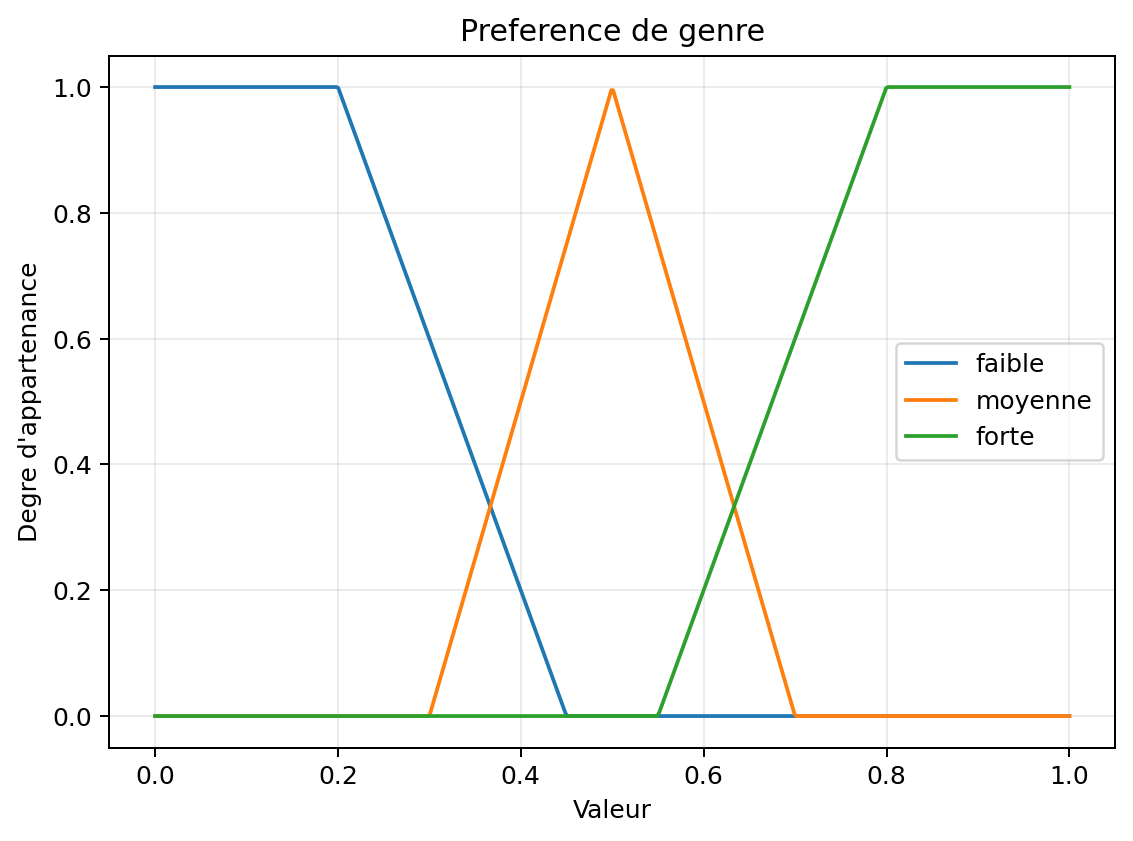
\includegraphics[width=0.82\textwidth]{membership_genre_preference.png}
\caption{Fonctions d'appartenance de la preference de genre.}
\label{fig:membership_genre_preference}
\end{figure}

\begin{figure}[H]
\centering
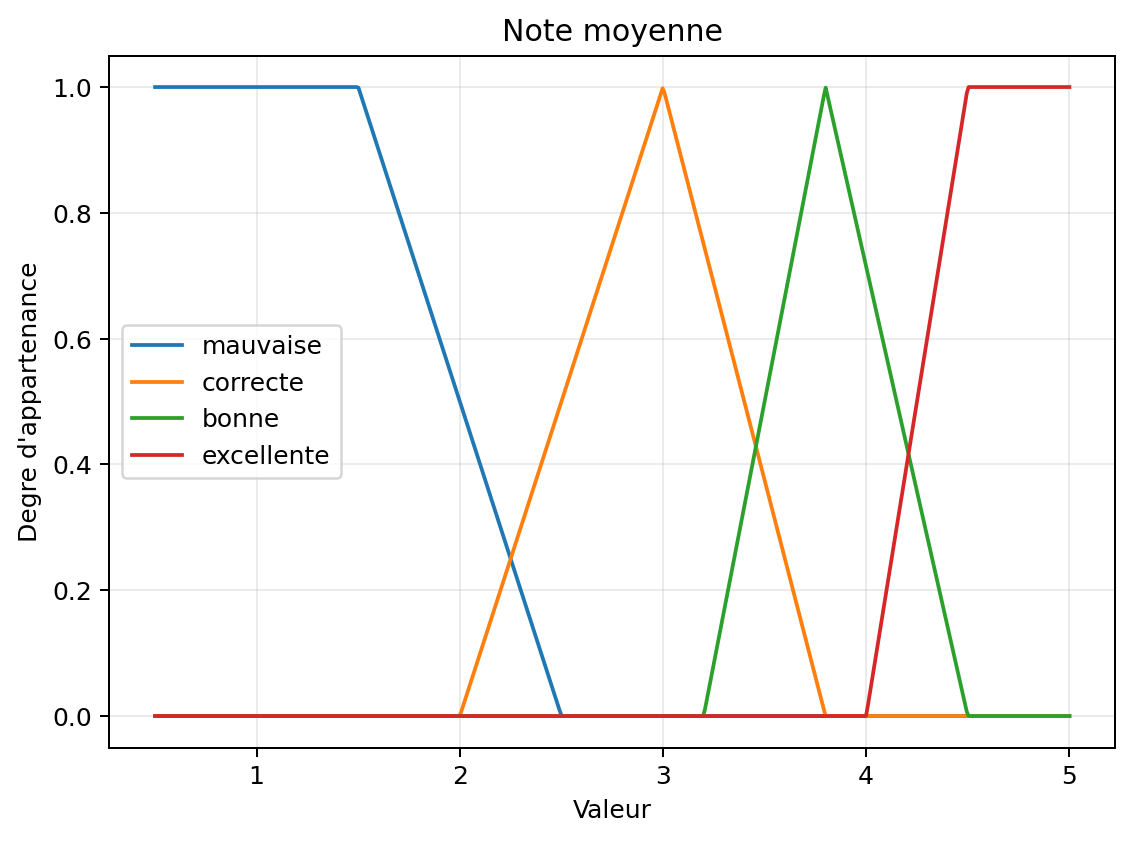
\includegraphics[width=0.82\textwidth]{membership_average_rating.png}
\caption{Fonctions d'appartenance de la note moyenne.}
\label{fig:membership_average_rating}
\end{figure}

\begin{figure}[H]
\centering
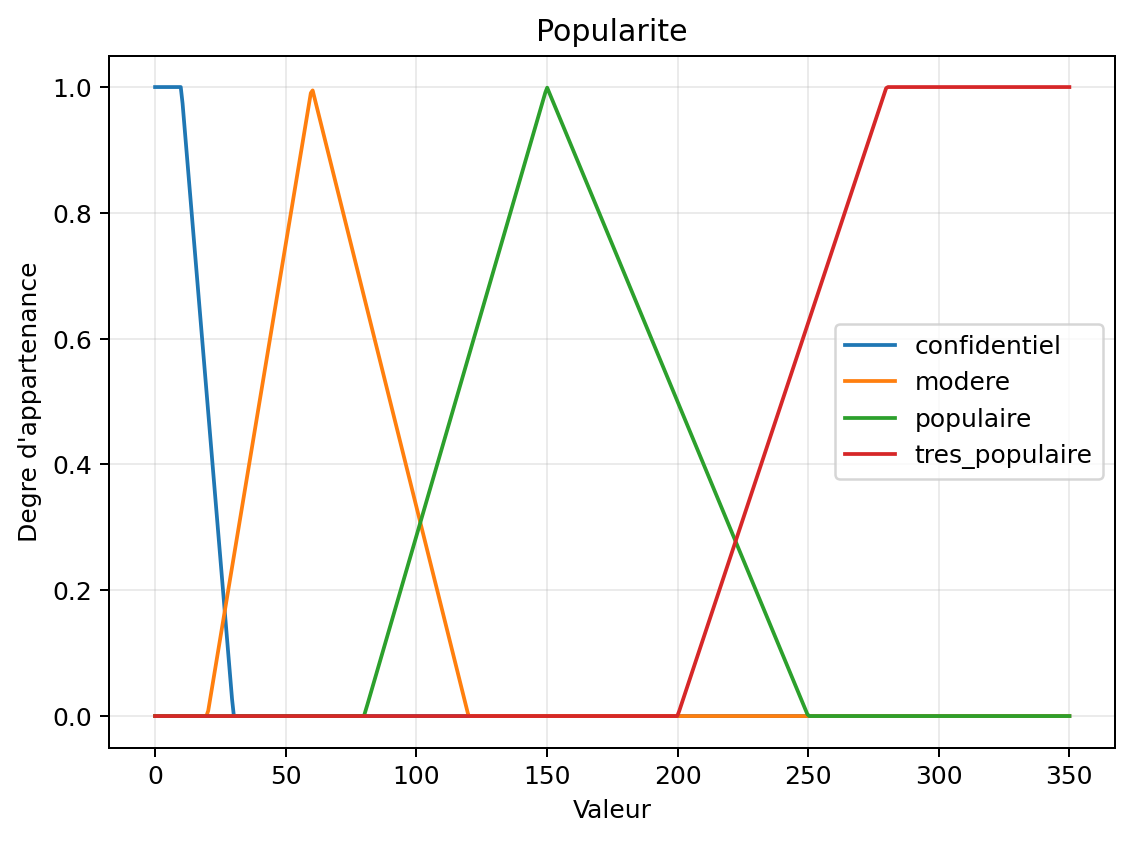
\includegraphics[width=0.82\textwidth]{membership_popularity.png}
\caption{Fonctions d'appartenance de la popularite.}
\label{fig:membership_popularity}
\end{figure}

\begin{figure}[H]
\centering
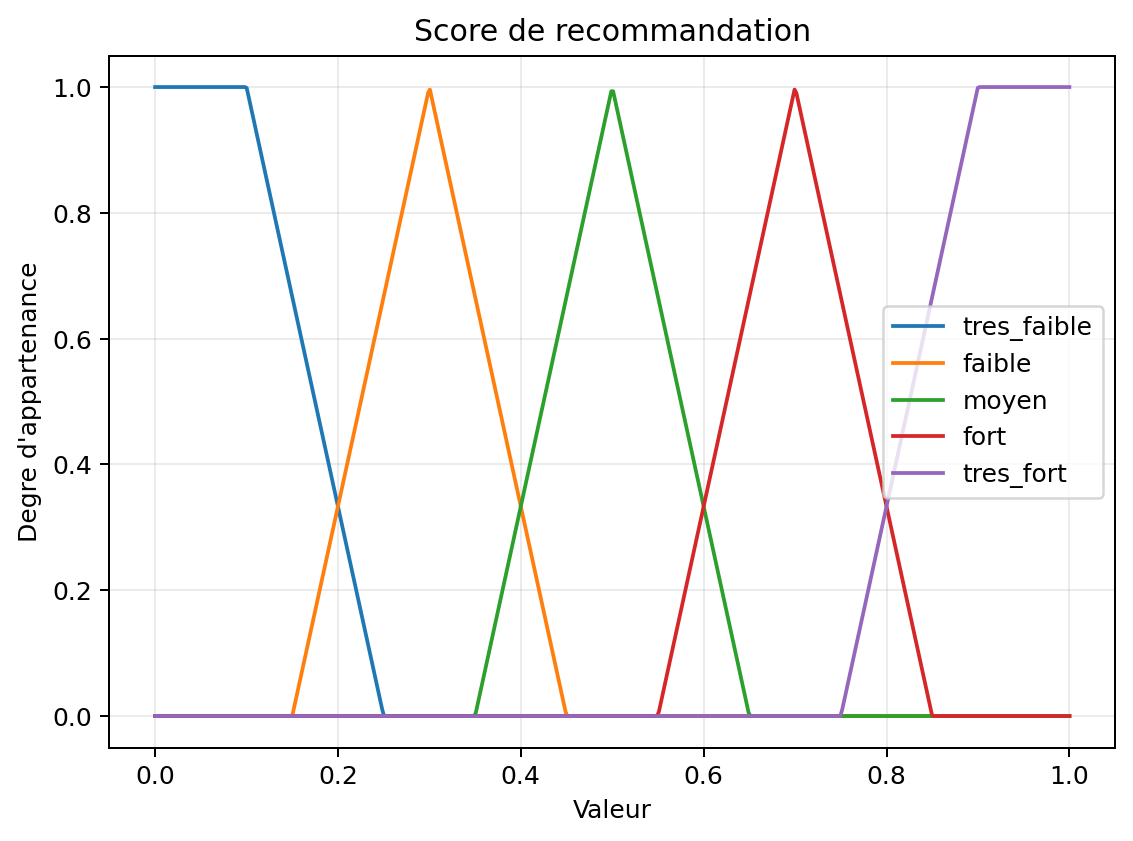
\includegraphics[width=0.82\textwidth]{membership_recommendation_score.png}
\caption{Fonctions d'appartenance du score de recommandation.}
\label{fig:membership_recommendation_score}
\end{figure}
\FloatBarrier

\subsection{Base de regles minimale}

\begin{table}[H]
\centering
\caption{Base de regles Mamdani minimale.}
\label{tab:rules}
\scriptsize
\begin{tabular}{@{}p{0.08\textwidth}p{0.59\textwidth}p{0.18\textwidth}@{}}
\toprule
Regle & Antecedents & Consequence \\
\midrule
R1 & preference forte, note excellente, popularite tres populaire & tres fort \\
R2 & preference forte, note excellente, popularite confidentiel & fort \\
R3 & preference forte, note bonne, popularite populaire & fort \\
R4 & preference moyenne, note excellente, popularite tres populaire & fort \\
R5 & preference moyenne, note bonne, popularite modere & moyen \\
R6 & preference faible, note excellente, popularite tres populaire & moyen \\
R7 & preference forte, note mauvaise, popularite populaire & faible \\
R8 & preference faible, note mauvaise, popularite confidentiel & tres faible \\
\bottomrule
\end{tabular}
\end{table}

Cette base de regles est volontairement compacte. Elle suffit a demontrer le raisonnement flou tout en gardant chaque decision explicable.

\subsection{Agregation et defuzzification}

Le moteur Mamdani utilise le minimum pour combiner les antecedents d'une regle, puis le maximum pour agreger les sorties activees. La defuzzification est realisee par centroide, conformement au parametrage \texttt{defuzzification\_method: centroid}. La figure d'inference de la section 9 illustre cette surface agregee et la position du centroide.

La section suivante precise comment les preferences utilisateur, souvent imprecises, sont projetees vers ces variables linguistiques.

\section{Modelisation des preferences imprecises}

Le coeur du sujet porte sur la maniere de representer une preference qui n'est pas parfaitement numerique. Le systeme distingue explicitement la saisie utilisateur de son exploitation par le moteur flou.

\subsection{Trois modes de saisie}

Le profil utilisateur accepte trois formes. La premiere est linguistique, par exemple \texttt{Sci-Fi=forte}, et correspond a \texttt{LinguisticGenrePreference}. La deuxieme est un intervalle, par exemple \texttt{Action=0.5..0.8}, represente par \texttt{IntervalGenrePreference}. La troisieme est crisp, c'est-a-dire une valeur ponctuelle dans $[0,1]$.

Dans la version actuelle, les valeurs crisp sont acceptees seulement lorsque ce mode est choisi explicitement. Cette contrainte evite de diluer l'objectif du projet, qui est de mettre en avant les preferences imprecises plutot qu'une simple notation numerique.

\subsection{Projection vers des degres d'appartenance}

La fonction \texttt{Fuzzifier.fuzzify\_imprecise\_value} realise la transformation vers les degres flous. Pour un terme linguistique, le systeme calcule l'alpha-cut a 0.5 du terme correspondant, puis projette cet intervalle sur toutes les fonctions d'appartenance de la variable. Pour un intervalle explicite, la projection prend le maximum atteint par chaque terme sur la plage. Pour une valeur crisp, la fuzzification classique est appliquee.

Par exemple, une preference \texttt{forte} n'est pas remplacee par une constante unique. Elle active la zone du terme \emph{forte} et peut conserver un chevauchement avec le terme voisin. De meme, l'intervalle $0.5..0.8$ peut activer simultanement \emph{moyenne} et \emph{forte}. Cette approche rejoint l'idee generale de la logique floue : l'incertitude est propagee plutot qu'effacee.

\subsection{Agregation multi-genres}

Un film MovieLens peut appartenir a plusieurs genres. La methode \texttt{genre\_preference\_for\_movie} compare donc les genres du film aux preferences declarees dans le profil. Si aucun genre ne correspond, le systeme retourne un etat \emph{inconnu}, distinct d'une preference faible. Si plusieurs genres correspondent, la strategie par defaut calcule la moyenne des forces de preference. Une strategie par maximum reste disponible, mais elle est moins nuancee, car elle peut masquer une preference faible associee a un autre genre. Une extension naturelle consisterait a utiliser des operateurs OWA pour controler plus finement l'optimisme ou la prudence de cette aggregation \cite{yager1988}.

Ainsi, avec un profil $\{\text{Sci-Fi}: \text{forte}, \text{Action}: 0.5..0.8\}$, un film \emph{Action|Sci-Fi} combine une preference linguistique forte et un intervalle moyen-fort. Le systeme conserve cette nuance jusqu'a la fuzzification, puis active les regles Mamdani selon les degres obtenus.

Une fois les preferences representees, il reste a organiser leur passage dans la chaine complete de recommandation. C'est l'objet de la section suivante.

\section{Pipeline de recommandation}

Le pipeline transforme un profil utilisateur et un catalogue de films en liste Top-N expliquee. Il est implemente principalement dans \texttt{pipeline\_factory.py}, \texttt{fuzzy\_recommender.py} et \texttt{explanation\_engine.py}.

\begin{figure}[H]
\centering
\resizebox{0.48\textwidth}{!}{%
\begin{tikzpicture}[
  >=Stealth,
  recstep/.style={draw=black!60, rounded corners, thick, fill=blue!8, minimum width=5.3cm, minimum height=0.82cm, align=center, drop shadow},
  arr/.style={->, thick}
]
  \node[recstep] (p) {Profil utilisateur};
  \node[recstep, below=0.45cm of p] (pre) {Pre-filtrage par genres};
  \node[recstep, below=0.45cm of pre] (fuz) {Fuzzification};
  \node[recstep, below=0.45cm of fuz] (inf) {Inference Mamdani};
  \node[recstep, below=0.45cm of inf] (agg) {Agregation};
  \node[recstep, below=0.45cm of agg] (def) {Defuzzification};
  \node[recstep, below=0.45cm of def] (score) {Score};
  \node[recstep, below=0.45cm of score] (rank) {Classement};
  \node[recstep, below=0.45cm of rank] (top) {Top-N};
  \node[recstep, below=0.45cm of top] (exp) {Explications};
  \foreach \a/\b in {p/pre,pre/fuz,fuz/inf,inf/agg,agg/def,def/score,score/rank,rank/top,top/exp}
    \draw[arr] (\a) -- (\b);
\end{tikzpicture}
}
\caption{Pipeline vertical de recommandation.}
\label{fig:pipeline}
\end{figure}

La premiere etape construit le profil. Si des preferences explicites sont fournies, elles priment sur l'historique MovieLens. Sinon, le profil est derive des notes de l'utilisateur par genre. Cette construction est centralisee dans \texttt{build\_profile}.

La deuxieme etape effectue un pre-filtrage par genre. Le seuil V1 est fixe a $0.2$ dans la configuration. Les films sans popularite connue sont exclus du Top-N afin d'eviter qu'une valeur manquante soit interpretee comme une faible popularite reelle.

La troisieme etape calcule les entrees crisp ou imprecises du moteur flou : preference de genre, note moyenne et popularite. Ces valeurs sont fuzzifiees selon les variables linguistiques de la V1.

La quatrieme etape active la base de regles Mamdani. Chaque regle produit un degre d'activation et une consequence sur la variable de sortie. Les sorties sont agregees par maximum, puis defuzzifiees par centroide pour produire un score dans $[0,1]$.

Enfin, les films sont tries par score decroissant, puis par popularite, note moyenne et titre. L'objet de recommandation conserve aussi les entrees floues et les regles activees, ce qui permet a \texttt{ExplanationEngine} de generer une trace lisible.

Ce pipeline etant defini, la section suivante presente les choix techniques qui ont permis de l'implementer et de le tester.

\section{Implementation}

L'implementation vise deux objectifs : rester proche du modele theorique et offrir une base testable. Les choix techniques sont donc simples, largement disponibles et adaptes a une execution locale.

\subsection{Stack technologique}

Le projet est implemente en Python. Le fichier \texttt{pyproject.toml} declare une compatibilite \texttt{Python >=3.10}. Les principales dependances sont \texttt{pandas} pour la manipulation des tables MovieLens, \texttt{NumPy} pour les calculs numeriques, \texttt{PyYAML} pour la configuration, \texttt{Tkinter} pour la GUI, \texttt{Matplotlib} pour les figures et \texttt{pytest} pour les tests. Le paquet \texttt{click} fournit l'interface CLI.

\subsection{Organisation du code}

L'arborescence du dossier \texttt{src/} suit les modules presentes dans l'architecture :
\begin{verbatim}
src/
  data_manager/    chargement, validation, preprocessing
  fuzzy/           ensembles flous, variables, Mamdani, defuzzification
  recommender/     profils, prefiltrage, scoring, explications
  evaluation/      metriques et protocole train/test
  ui/              commandes CLI et interface Tkinter
  visualization/   generation des courbes d'appartenance
\end{verbatim}

Cette organisation permet de tester separement les composants. Par exemple, la defuzzification peut etre verifiee sans lancer l'interface graphique, et l'evaluation peut reutiliser un moteur deja construit.

\subsection{Configuration externalisee}

Le fichier \texttt{config/fuzzy\_config.yaml} contient les variables linguistiques, les fonctions d'appartenance, les regles, la methode de defuzzification, le seuil de pre-filtrage et les chemins de donnees. Cette externalisation ameliore la reproductibilite : les valeurs du rapport peuvent etre relancees avec le meme fichier de configuration. Elle facilite aussi les ajustements : ajouter des regles ou modifier une fonction d'appartenance ne demande pas de recompilation ni de modification des interfaces.

\subsection{Execution}

Les commandes principales sont les suivantes :
\begin{verbatim}
python main.py recommend --user-id 1 --top-n 10 \
  --set-genre "Sci-Fi=forte,Action=moyenne" --explain

python main.py gui --data-dir data/movie

python main.py evaluate --user-id 1 --top-n 10
\end{verbatim}

La premiere commande produit un Top-N explique, la deuxieme lance l'interface graphique, et la troisieme calcule les metriques d'evaluation. Ces commandes constituent le point d'entree des experiences de la section 9.

La section suivante presente les interfaces qui rendent ces operations accessibles a l'utilisateur.

\section{Interfaces utilisateur}

Deux interfaces sont proposees. La CLI sert a reproduire rapidement les experiences et a automatiser les tests. La GUI sert a manipuler les preferences de maniere visuelle et a observer les courbes d'appartenance.

\subsection{Interface CLI}

L'interface en ligne de commande est exposee par \texttt{main.py}. Elle regroupe notamment les sous-commandes \texttt{recommend}, \texttt{evaluate}, \texttt{dataset-stats} et \texttt{gui}. La commande \texttt{recommend} accepte un identifiant utilisateur, un nombre de recommandations et des preferences explicites. Elle peut aussi afficher l'explication des regles activees.

\begin{figure}[H]
\centering
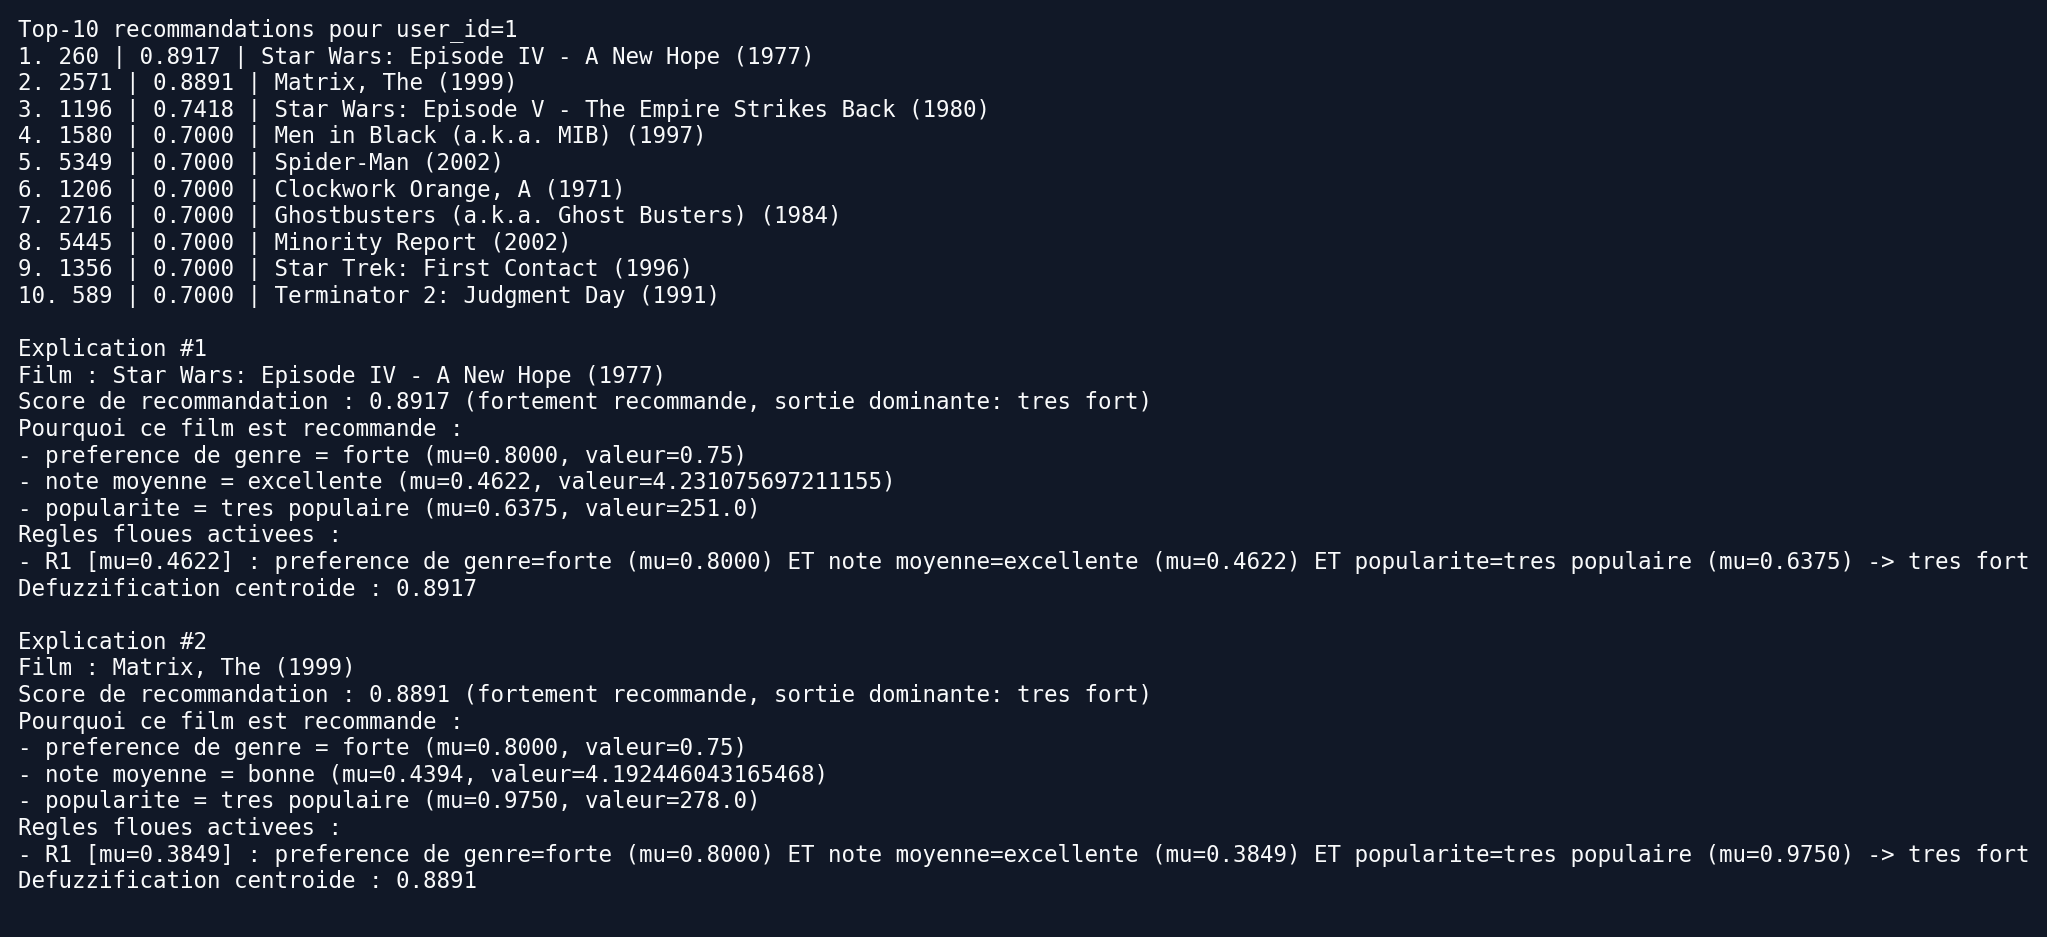
\includegraphics[width=0.85\textwidth]{cli_recommend.png}
\caption{Capture de la commande CLI \texttt{recommend} pour \texttt{user\_id=1}. La sortie affiche le Top-N, le score defuzzifie et une trace textuelle des regles Mamdani activees pour les premieres recommandations.}
\label{fig:cli_recommend}
\end{figure}

La CLI est particulierement utile pour verifier la reproductibilite des resultats, car les memes parametres peuvent etre relances sans interaction graphique.

\subsection{Interface GUI}

L'interface graphique Tkinter est organisee en trois zones. La premiere zone permet de choisir l'utilisateur, le nombre de recommandations et le dossier MovieLens. Le bouton \emph{Changer dossier} permet de charger un autre dataset compatible. La deuxieme zone contient un notebook avec les onglets \emph{Preferences} et \emph{Courbes}. La troisieme zone affiche les films recommandes et la trace d'explication.

\begin{figure}[H]
\centering
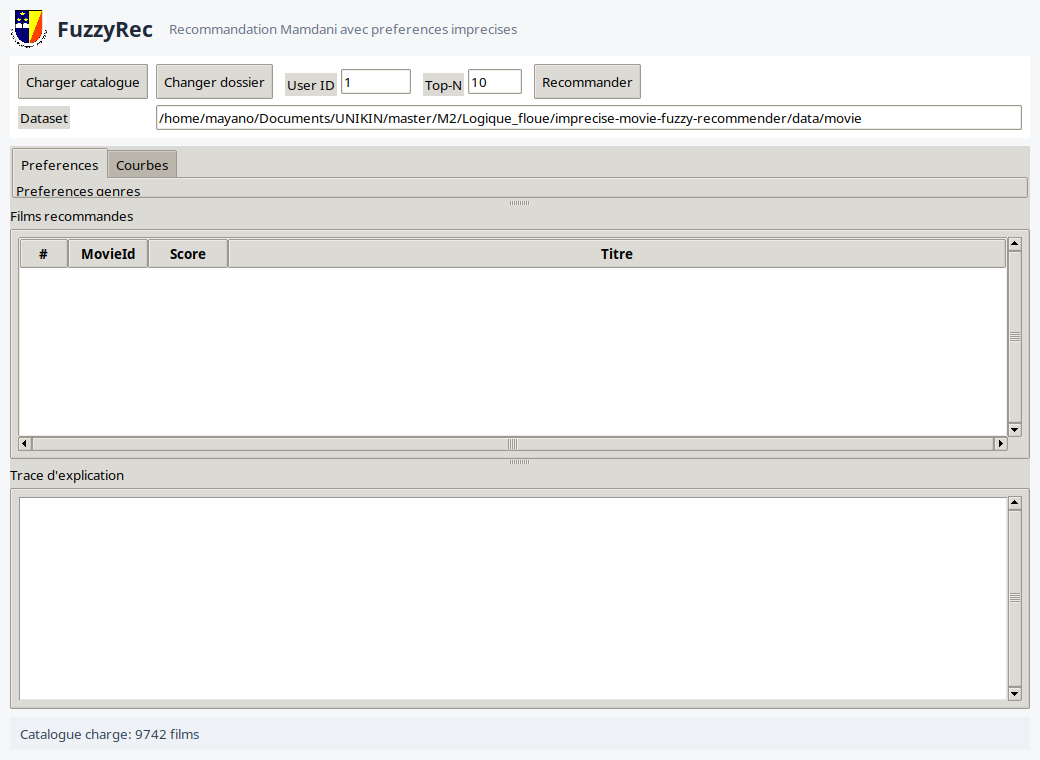
\includegraphics[width=0.85\textwidth]{gui_preferences.png}
\caption{Onglet des preferences : chaque genre dispose d'un curseur, d'un libelle linguistique dominant et d'une combobox permettant de choisir le mode linguistique, crisp ou intervalle.}
\label{fig:gui_preferences}
\end{figure}

\begin{figure}[H]
\centering
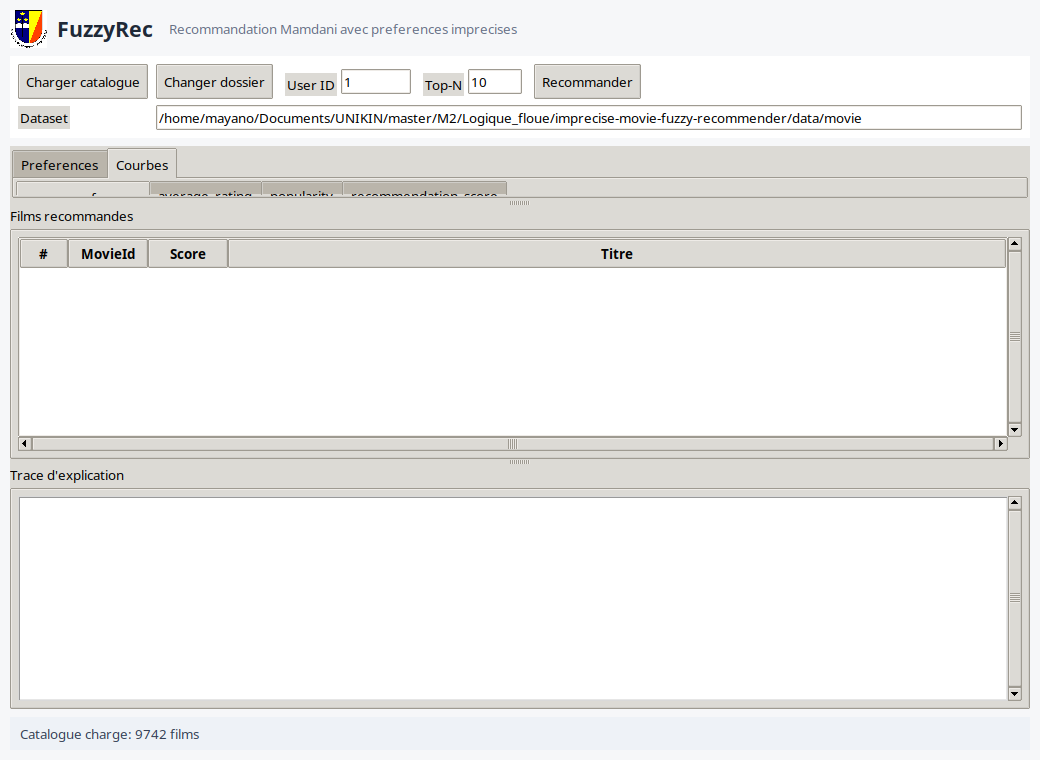
\includegraphics[width=0.85\textwidth]{gui_courbes.png}
\caption{Onglet des courbes : les fonctions d'appartenance des variables linguistiques sont integrees dans la GUI afin de rendre visible la transformation des preferences.}
\label{fig:gui_courbes}
\end{figure}

\begin{figure}[H]
\centering
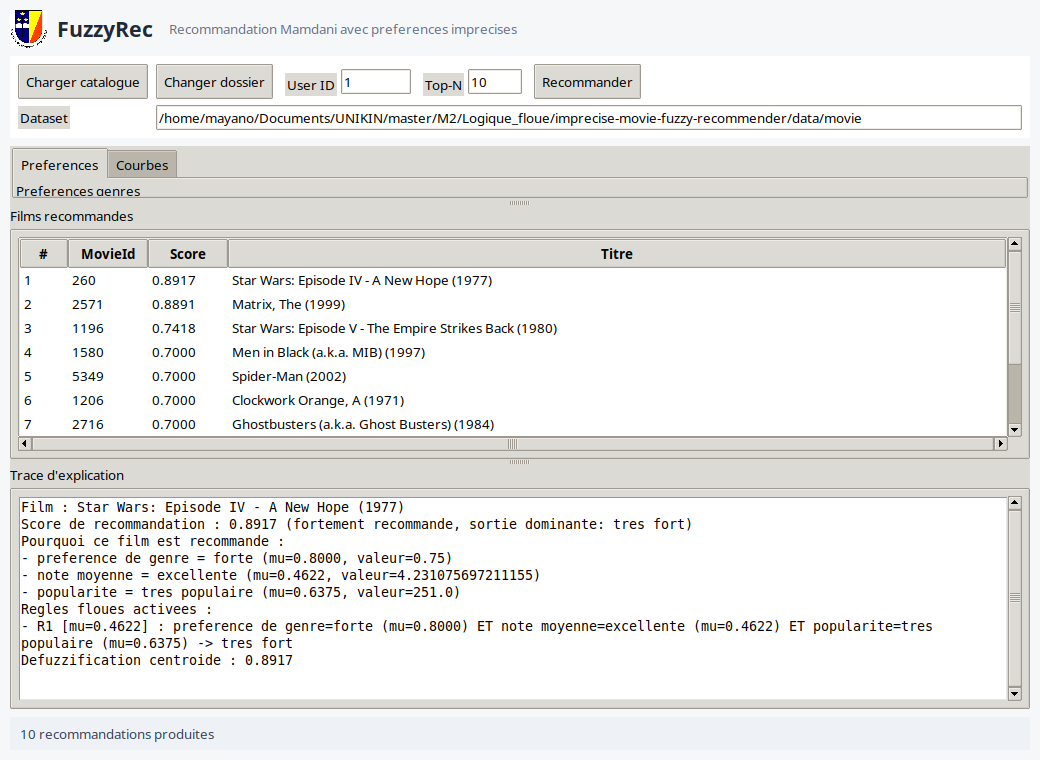
\includegraphics[width=0.85\textwidth]{gui_resultats.png}
\caption{Zone des resultats : le Top-N est affiche dans un tableau et la trace d'explication detaille les degres flous et les regles activees pour la recommandation selectionnee.}
\label{fig:gui_resultats}
\end{figure}
\FloatBarrier

Deux problemes UX initiaux ont ete corriges. D'abord, la saisie par texte a ete remplacee par des curseurs par thematique, ce qui rend les preferences plus directes. Ensuite, la coherence entre les modes numerique, linguistique et intervalle est assuree par une combobox par genre. Ainsi, la GUI ne force pas l'utilisateur a connaitre la syntaxe CLI pour experimenter.

Ces interfaces permettent maintenant de produire les resultats experimentaux presentes dans la section suivante.

\section{Resultats et evaluation}

Cette section presente des resultats issus d'executions reelles du projet. Les commandes ont ete lancees sur le dossier \texttt{data/movie}, qui correspond au jeu MovieLens small utilise dans le projet.

\subsection{Protocole experimental}

Le protocole utilise le dataset MovieLens \texttt{ml-latest-small} \cite{harper2015}. Le profil d'exemple est \texttt{user\_id=1}, avec les preferences explicites \texttt{Sci-Fi=forte,Action=moyenne}. Le nombre de recommandations est fixe a $5$ pour l'exemple detaille et a $10$ pour l'evaluation. Le seuil de pre-filtrage est celui de la configuration V1, soit $0.2$.

\subsection{Exemple de recommandation detaillee}

La commande executee est :
\begin{verbatim}
python main.py recommend --user-id 1 --top-n 5 \
  --set-genre "Sci-Fi=forte,Action=moyenne" --explain --data-dir data/movie
\end{verbatim}

Le Top-5 obtenu est presente dans le tableau suivant.

\begin{table}[H]
\centering
\caption{Top-5 obtenu pour \texttt{user\_id=1}.}
\label{tab:top5}
\small
\begin{tabular}{@{}clc@{}}
\toprule
Rang & Titre & Score \\
\midrule
1 & Star Wars: Episode IV - A New Hope (1977) & 0.8917 \\
2 & Matrix, The (1999) & 0.8891 \\
3 & Star Wars: Episode V - The Empire Strikes Back (1980) & 0.7418 \\
4 & Men in Black (a.k.a. MIB) (1997) & 0.7000 \\
5 & Spider-Man (2002) & 0.7000 \\
\bottomrule
\end{tabular}
\end{table}

Pour la premiere recommandation, la trace indique une preference de genre forte avec $\mu=0.8000$, une note moyenne excellente avec $\mu=0.4622$ et une popularite tres populaire avec $\mu=0.6375$. La regle R1 est activee avec un degre $0.4622$ et produit la sortie \emph{tres fort}. La defuzzification par centroide donne le score $0.8917$.

\subsection{Illustration de l'inference Mamdani}

\begin{figure}[H]
\centering
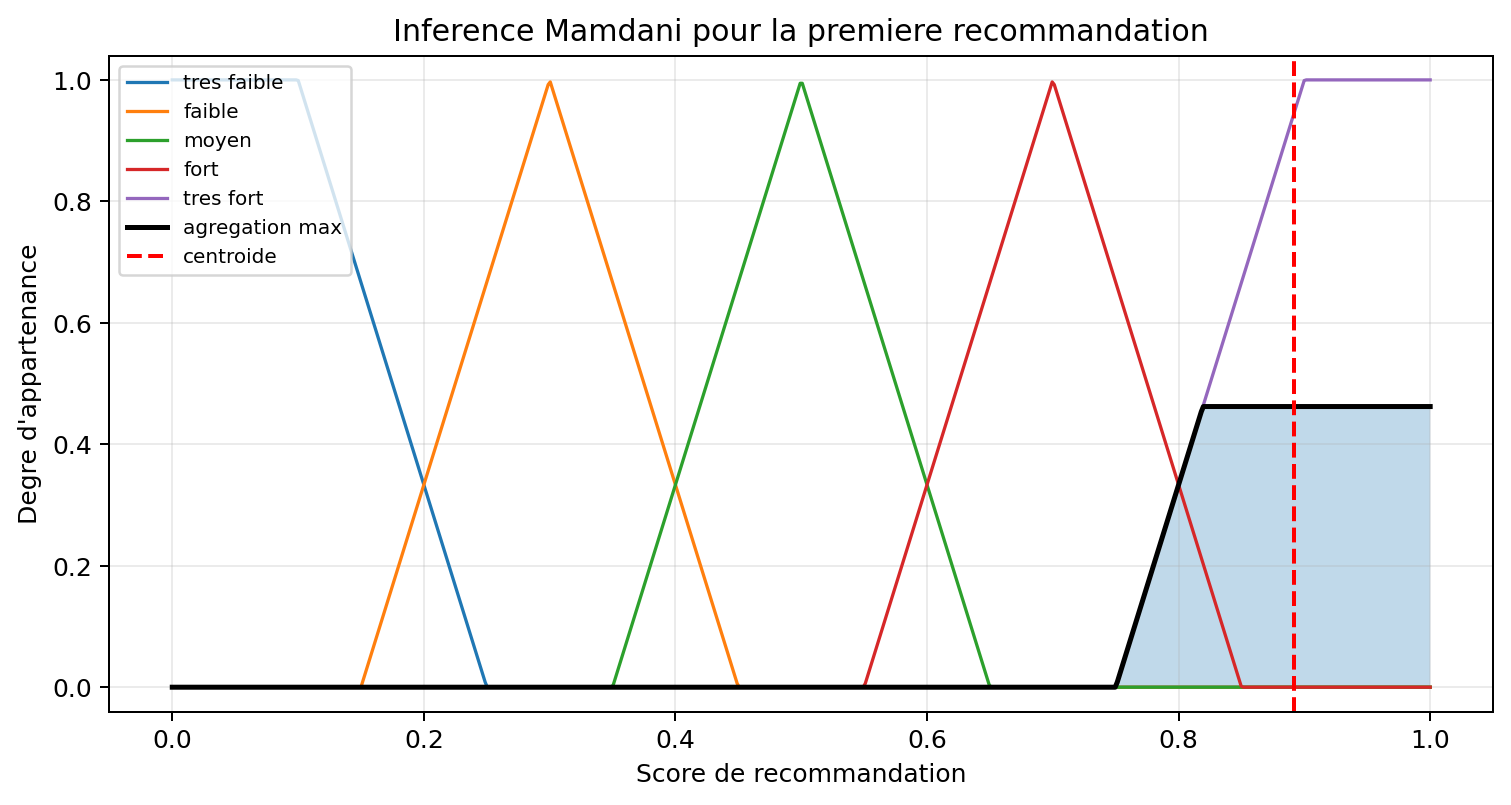
\includegraphics[width=0.85\textwidth]{exemple_inference_mamdani.png}
\caption{Illustration de l'inference Mamdani pour la premiere recommandation : les sorties tronquees sont agregees par maximum, puis le centroide fournit le score final.}
\label{fig:inference_mamdani}
\end{figure}

La figure montre que la recommandation ne depend pas d'une seule condition. Elle resulte de la combinaison des degres d'appartenance et de l'agregation des consequences floues.

\subsection{Metriques d'evaluation}

Le protocole \texttt{evaluate} realise un decoupage temporel des notes de l'utilisateur. Les notes anciennes construisent le profil, tandis que les notes recentes servent de reference. Les resultats suivants proviennent de trois executions reelles avec \texttt{top-n=10}.

\begin{table}[H]
\centering
\caption{Metriques d'evaluation pour trois utilisateurs MovieLens.}
\label{tab:metrics}
\small
\begin{tabular}{@{}ccccc@{}}
\toprule
Utilisateur & Precision@10 & Recall@10 & Coverage & Diversite \\
\midrule
1 & 0.2000 & 0.0526 & 0.0010 & 0.7746 \\
2 & 0.0000 & 0.0000 & 0.0010 & 0.7746 \\
3 & 0.0000 & 0.0000 & 0.0010 & 0.6589 \\
\bottomrule
\end{tabular}
\end{table}

Ces valeurs doivent etre interpretees comme une verification experimentale de la chaine de calcul plutot que comme une optimisation finale. La base de regles V1 est volontairement minimale, ce qui limite la couverture decisionnelle.

\subsection{Tests automatises}

La commande \texttt{./.venv/bin/pytest -q} a ete executee avant la redaction finale. Le resultat obtenu est :
\begin{verbatim}
96 passed in 7.79s
\end{verbatim}
Les tests couvrent les fonctions d'appartenance, la fuzzification, la base de regles, l'inference, la defuzzification, le repository MovieLens, le pipeline de recommandation, les explications, les metriques, la CLI et les composants GUI.

Les resultats confirment que la V1 est executable et testee. La section suivante discute ce que cette version demontre, mais aussi ce qu'elle ne pretend pas encore resoudre.

\section{Discussion, conclusion et perspectives}

\subsection{Discussion}

La principale force du systeme est son interpretabilite. Chaque recommandation conserve les degres d'appartenance, les regles activees et le score defuzzifie. Cette trace permet d'expliquer pourquoi un film est classe en tete, ce qui est plus transparent qu'un simple score opaque.

Le deuxieme apport est la prise en charge de plusieurs modes d'expression des preferences : linguistique, intervalle et crisp. Le systeme separe la representation imprecise de la decision finale. La preference n'est donc pas immediatement reduite a une note unique ; elle est projetee vers des degres flous et combinee par le moteur Mamdani.

Les limites sont egalement claires. La base V1 contient huit regles seulement. Elle suffit pour demontrer le principe, mais ne couvre pas toutes les situations possibles. Le pre-filtrage par genre reste simple et ne tient pas encore compte des tags ou de la recence. Enfin, la popularite est utilisee comme critere global, sans personnalisation profonde selon le comportement de chaque utilisateur.

\subsection{Adequation au sujet}

Le sujet 12 demande un systeme de recommandation flou base sur les preferences imprecises des utilisateurs \cite{kasereka2026}. Le systeme repond a ce sujet sur quatre points. Premierement, il represente explicitement les preferences imprecises par termes linguistiques et intervalles. Deuxiemement, il utilise un moteur Mamdani interpretable pour convertir ces preferences en score de recommandation. Troisiemement, il applique le modele a un catalogue reel, MovieLens. Quatriemement, il fournit une CLI et une GUI permettant de reproduire les resultats et de visualiser les memberships.

\subsection{Perspectives}

La premiere perspective consiste a etendre la base de regles. Le fichier YAML contient deja une entree \texttt{intermediate} prevue pour une V2 plus riche. La deuxieme perspective est l'integration des tags MovieLens, qui permettraient de modeliser des preferences thematiques plus fines que les genres. Une representation semantique floue, proche des travaux sur les ontologies floues \cite{bobillo2011}, pourrait alors relier genres, mots-cles et concepts narratifs. La troisieme perspective concerne la recence : un film ancien et un film recent pourraient etre traites differemment selon le profil. Enfin, les parametres des fonctions d'appartenance pourraient etre appris ou ajustes automatiquement a partir des historiques utilisateurs.

\subsection{Conclusion}

Ce travail a montre qu'un systeme de recommandation peut traiter des preferences vagues sans les convertir immediatement en notes rigides. En combinant variables linguistiques, preferences imprecises, inference de Mamdani et explications, la solution proposee fournit une V1 coherent, interpretable et reproductible sur MovieLens. Les resultats experimentaux restent modestes, mais ils valident l'objectif principal : construire une chaine complete reliant l'expression naturelle de la preference a une recommandation floue expliquee.


\newpage
\bibliographystyle{plain}
\bibliography{references}

\newpage
\appendix
\section{Code source}
L'integralite du code source, des tests et de la configuration est publiee sous licence libre dans le depot public suivant : \github. Le lecteur y trouvera les instructions d'installation, le jeu de donnees MovieLens utilise et les scripts permettant de reproduire l'ensemble des resultats presentes dans ce rapport.

\end{document}
